\documentclass{article}
\usepackage{amsmath}
\usepackage{amssymb}
\usepackage{tikz}
\usepackage[ruled]{algorithm2e}
\usepackage{pgfplots}

\usepackage[export]{adjustbox}
\usepackage[linktoc=all]{hyperref}

\hypersetup{pdfborder = {0 0 0}} % no red box on table of contents link

\def\arraystretch{1.3} % spacing of rows

\begin{document}
\begin{titlepage}

  \newcommand{\HRule}{\rule{\linewidth}{0.5mm}}

  \center

  \begin{figure}
    \centering
    
\includegraphics[scale=0.75]{logo.png}
  \end{figure} 
  
  \textsc{\Large Calcul haute performance} \\[0.5cm]

  \HRule\\[0.5cm]

  {\huge\bfseries Rendu "photo-r\'ealiste" avec illumination globale}\\[0.3cm]

  \HRule\\[2.4cm]

  \begin{minipage}{0.4\textwidth}
		\begin{flushleft}
			\large
      \textit{Auteurs}\\[0.3cm]
      \textsc{Antoine Mas} \\[0.1cm]
      \textsc{Yoann Valeri} \\[0.1cm]
		\end{flushleft}
	\end{minipage}
  ~
  \begin{minipage}{0.4\textwidth}
		\begin{flushright}
			\large
      \textit{Encadrants}\\[0.3cm]
      \textsc{S. Moustafa} \\[0.1cm]
      \textsc{C. Makassikis} \\[0.1cm]
		\end{flushright}
	\end{minipage}

  \vspace*{\fill}
  \textsc{\today}

\end{titlepage}

\tableofcontents

\newpage

\section{Introduction}

\subsection{Path-tracer}
\paragraph{}
Le path-tracing est une m\'ethode de calcul servant \`a effectuer le rendu d'une image de synth\`ese. 
Aussi appel\'e "technique d'illumination globale", on calcule la quantit\'e de lumi\`ere vers un piel en utilisant un
processus de Monte-Carlo, qui se fait en lancant un grand nombre de rayon qui rebondissent dans la sc\`ene afin d'obtenir une illumination moyenne.
Cela simule naturellement plusieurs effets photos-r\'ealiste.

\subsection{Sujet du projet}
\paragraph{}
Ce projet consiste donc en la parall\'elisation d'un "path-tracer". 
Ce proc\'ed\'e est assez long si effectu\'e de mani\`ere s\'equentiel, 
c'est-\`a-dire si un seul processus s'occupe de faire tout les calculs et de faire le rendu.
Ainsi, pour am\'eliorer le temps global, il nous est propos\'e plusieurs moyen de parall\'eliser le code, que nous allons utiliser ensemble pour essayer de r\'eduire au plus possible le temps de calcul global :

\begin{enumerate}
  \item Le premier moyen abord\'e est OpenMPI, une API permettant d'effectuer un calcul sur plusieurs processeurs distants ou d'une m\^eme machine.
  \item Le second est OpenMP, une API qui elle joue sur la cr\'eation de threads, chacun effectuant un certain nombre d'op\'erations en parall\`ele d'autres threads.
  \item Enfin, nous allons utiliser les instructions SIMD (OpenMP + fonctions intrins\`eques), qui permettent de vectoriser des calculs, et donc de pouvoir effectuer plusieurs op\'erations sur un vecteur en utilisant le mêême temps que si l'on en faisant qu'une seule.
\end{enumerate}

\subsection{Modification du projet}
\paragraph{}
Dans ce projet, deux cas de test nous sont donn\'es : calculer une image de taille 320 * 200 avec 200 samples, et une seconde image de taille 3840 * 2160 avec 5000 samples.
Nous avons calcul\'e que pour faire la seconde image, il nous faudrait au minimum 150 heures.
Ainsi, pour pouvoir effectuer des calculs \`a partir d'une image plus grosse, mais en ayant le temps de calcul s\'equentiel dans un temps raisonnable, nous avons d\'ecid\'e d'ajouter le calcul d'une image 1280 * 1024 avec 200 samples.

\newpage

\section{Parall\'elisation OpenMPI}

\subsection{Probl\'ematique}

\paragraph{}
Pour effectuer nos tests, nous utilisons les machines mises \`a disposition par la PPTI et 
limitons nos programmes \`a l'utilisation des machines d'une seule salle, soit au maximum 64 coeurs (à raison de 16 machines avec 4 coeurs chacune).

\paragraph{}
Le probl\`eme central de cette partie OpenMPI va donc \^etre de faire communiquer ces 64 processus pour effectuer le travail
le plus rapidement possible. Nous allons maintenant voir de mani\`ere pratique quels sont les probl\`emes qu'il faudra r\'esoudre pour 
mener \`a bien ce projet.

\subsection{Difficult\'ees rencontr\'ees}

\paragraph{Cr\'eation des t\^aches : }
Les images \'etant trop longues \`a calculer par un seul processus, il nous faut r\'epartir les t\^aches entre diff\'erentes processus,
c'est-\`a-dire cr\'eer un ensemble de plus petites t\^aches que chaque processus devra effectuer de son c\^ot\'e. 

\paragraph{La r\'epartition dynamique : }
Le temps de calcul de deux t\^aches peut \^etre radicalement diff\'erent, il nous faut faire une
r\'epartition dynamique.

\paragraph{Données : }
Un des probl\`emes li\'es \`a ce type d'\'equilibrage de charge est la r\'epartition des donn\'ees : quel processus aura quelles donn\'ees ?

\paragraph{Partage des t\^aches : }
Le probl\`eme suivant est de savoir \`a quel processus demander des t\^aches et combien de t\^ache donner.
On cherche \`a \'eviter les communications inutiles entre des processus ne pouvant pas se donner de t\^ache
et ne pas avoir les processus rapide n'aidant pas les processus lents.

\paragraph{Fin des calculs : }
On doit trouver un moment \`a partir duquel un processus suppose que tous les calculs (ou presque) ont \'et\'e fait
et arr\^ete de chercher de nouvelles t\^aches.

\paragraph{Récupération de l'image : }
Le dernier probl\`eme concerne la mani\`ere dont chaque processus va communiquer pour rassembler les donn\'ees. 

\newpage

\subsection{Solution choisie}

\paragraph{}
Pour tout le projet, nous avons choisi d'utiliser les fonctions vu en cours et d'optimiser les communications entre les processus.

\paragraph{Cr\'eation des t\^aches : }
Une premi\`ere id\'ee que nous avons eu est de faire un d\'ecoupage 1D par ligne. 
Cependant, cette solution peut s'av\'erer inefficace si le temps de calcul des lignes augmente.
Nous avons donc choisi de faire des t\^aches de pixels continus, avec un nombre de pixel d\'etermin\'e
en fonction du nombre de sample. Chaque t\^ache a un temps de calcul d'environ une seconde sur les machines de la PPTI. 
Pour nos tests, nous utilisons :
$$
  \text{Nombre de pixel par t\^ache} = \frac{5}{8} * \text{Nombre de sample}
$$
  
\paragraph{La r\'epartition dynamique : }
L'\'equilibrage que nous allons utiliser est un \'equilibrage de charge dynamique de type auto-r\'egul\'e.
Chaque processus a des t\^aches attribu\'ees au d"but du programme. Les t\^aches attribu\'ees pour un processus sont 
r\'epartis de manière cyclique pour \'eviter qu'une zone complexe à calculer soit donn\'ee au m\^eme processus.
Ensuite, si un processus est plus rapide que les autres il pourra voler des t\^aches \`a un processus plus lent.

\paragraph{Données : }
Pour r\'esoudre ce probl\`eme, nous faisons en sorte que chaque processus contienne un tableau d'information sur les tous les processus
ainsi que deux buffers, l'un contenant les r\'esultats qu'il a calculé et le second la liste des t\^aches qu'il a calcul\'e.
Ce tableau d'informations contient la position dans l'arbre des processus.(voir arbre \ref{fig:recup})
Il contient aussi plusieurs informations qui changeront pendant l'execution : le nombre de t\^ache assign\'ee et le nombre de t\^ache effectu\'ee par chaque processus distants.
Ces nombres sont des suppositions, sauf pour sa propre case qui contient les valeurs exactes. 
Ensuite, \`a chaque communication entre deux processus les tableaux des deux sont envoy\'ees, et les valeurs des cases correspondantes pour chaque chaque processus des deux sont mises \`a jour.

\begin{algorithm}[H]
  \SetKwInOut{Input}{input}

  \Input{T tableau initial d'informations des processus\newline
  U tableau re\c{c}u d'informations des processus \newline
  n le nombre de processus}

  \For{$i \leftarrow 0$ \KwTo $n$}{
    \If{T[i].nbDone $<$ U[i].nbDone}{
      \tcp{nbDone = nombre de t\^ache effectu\'ee}
      \tcp{nbAssigned = nombre de t\^ache assign\'ee}
      T[i].nbDone $\leftarrow$ U[i].nbDone\;
      T[i].nbAssigned $\leftarrow$ U[i].nbAssigned\;
    }
  }

  \caption{Mise \`a jour des informations processus}
\end{algorithm}

\paragraph{Partage des t\^aches : }
Ce probl\`eme est r\'esolu gr\^ace au tableau d'informations processus d\'ecrit pr\'ec\'edemment : 
lorsqu'un processus a peu de t\^ache \`a faire (en dessous d'un seuil), 
il va chercher dans le tableau le maximum de t\^aches encore \`a effecuter par les autres processus. Nous avons choisi de mettre notre seuil égal au nombre de processus.
Ensuite, s'il trouve une victime, il lui enverra un message pour lui demander des t\^aches, en même temps que son propre tableau T.
Le processus victime calculera le nombre de t\^ache \`a envoyer. 
Il renverra son tableau d'information avec plus ou moins de t\^aches \`a faire.
Le voleur mettra \`a jour son tableau, ajoutera ou non des t\^aches et continuera son execution.

\begin{algorithm}[H]
  \SetKwInOut{Input}{input}
  \Input{s le nombre de t\^ache assign\'ee du processus voleur\newline
    v le nombre de t\^ache assign\'ee du processus victime}

  \eIf{$ v < 3 $ {\bf or} $ v + 1 < s $}
  {
    \Return 0\;
  }
  {
    $ n \leftarrow \frac{v - s}{2} $ \;
    \eIf{$ n > 5 $}
    {
      \Return 5\;
    }
    {
      \Return $n$\;
    }
  }
  \caption{Calcul du nombre de t\^ache \`a envoyer}
\end{algorithm}

\paragraph{Fin des calculs : }
Lorsqu'un processus n'a plus de t\^ache \`a faire et qu'il n'est pas en train d'en voler, il commence la partie r\'ecup\'eration de l'image.
Nous definissons un seuil de partage des t\^aches de fa\c{c}on \`a ne pas finir alors que les autres processus ont encore beaucoup de t\^aches.

\paragraph{R\'ecup\'eration de l'image : }
Une id\'ee simple mais cependant inefficace avec notre mod\`ele est de faire un simple gather \`a la fin. 
Le probl\`eme est qu'ainsi, tous les processus rapides vont attendre les lents.
Nous avons choisi de r\'eimplementer notre gather en faisant une r\'ecup\'eration sous forme d'arbre binaire.
Un soucis induit par ce mode de r\'ecup\'eration est de savoir comment former l'arbre. \\
 - si l'on choisit de mani\`ere statique alors si une feuille met beaucoup de temps \`a calculer ses lignes, tout les autres vont l'attendre, sans rien faire ; \\
 - si l'on choisit un processus de mani\`ere dynamique, on a un grand nombre de communication pour former l'arbre.

Nous avons choisi de le faire de mani\'ere statique et d'orienter notre programme autour. Notre arbre est ordonn\'e de la mani\`ere suivante :

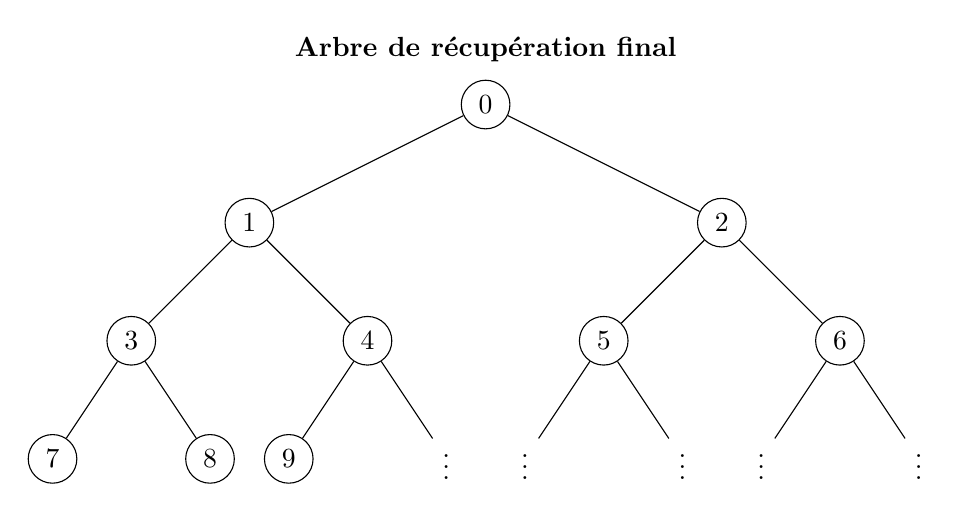
\begin{tikzpicture}
  [level/.style={sibling distance=60mm/#1}]
  \label{fig:recup}
\node[circle, draw]{0}
  child { node[circle, draw] {1}
    child { node[circle, draw] {3} 
      child { node[circle, draw] {7} }
      child { node[circle, draw] {8} }
    }
    child { node[circle, draw] {4}
      child { node[circle, draw] {9} }
      child { node {\vdots} }
    }
  }
  child { node[circle, draw] {2}
    child { node[circle, draw] {5} 
      child { node {\vdots} }
      child { node {\vdots} }
    }
    child { node[circle, draw] {6} 
      child { node {\vdots} }
      child { node {\vdots} }
    }
    }
;

\node[align=center, yshift=2em]
  {\textbf{Arbre de récupération final}};
\end{tikzpicture}

\paragraph{}
Donc chaque processus aura un parent (sauf le processus 0) et au maximum deux fils.
Il aura donc à calculer un ensemble de lignes, et les "fusionnera" aux donn\'ees que ses potentiels fils lui enverront. 
Ensuite, s'il a un parent, le processus lui enverra ses donn\'ees.
De cette mani\`ere, on assure qu'\`a la fin des envois/r\'ecup\'eration de donn\'ees, le processus 0 aura les donn\'ees de tout le monde pour rendre l'image.

\subsection{Analyse des performances}

\subsubsection{Mesure des performances}
\paragraph{}
Pour mesurer les temps de calcul de nos programmes, nous avons tout d'abord fait la diff\'erence entre le temps au d\'emarrage et le temps final. 
Cette m\'ethode a quelques d\'efaults, il se peut notamment que le programme mettent plus de temps à s'ex"cuter pour des raisons ext\'erieures (autre processus en arri\`ere-plan), et on peut donc obtenir des efficacit\'es anormales (certaines exécutions \'etait deux fois plus longue que la normale).
Cela posait aussi probl\`eme pour la grande image, il n'\'etait pas possible d'exécuter le programme en s\'equentiel (temps sup\'erieur \`a 150 heures).

Afin d'am\'eliorer la qualit\'e des tests, nous avons d\'ecid\'e de mesurer le temps pass\'e dans le calcul et de le comparer au temps total d'exécution.
Cela ne prends pas en compte l'am\'elioration possible gr\^ace aux caches processeurs mais nous permet d'avoir une meilleur visibilit\'e sur nos tests.

Tous les temps et calcul sont disponibles en annexe \ref{temps partie1}.

\newpage

\begin{figure}[h!]
  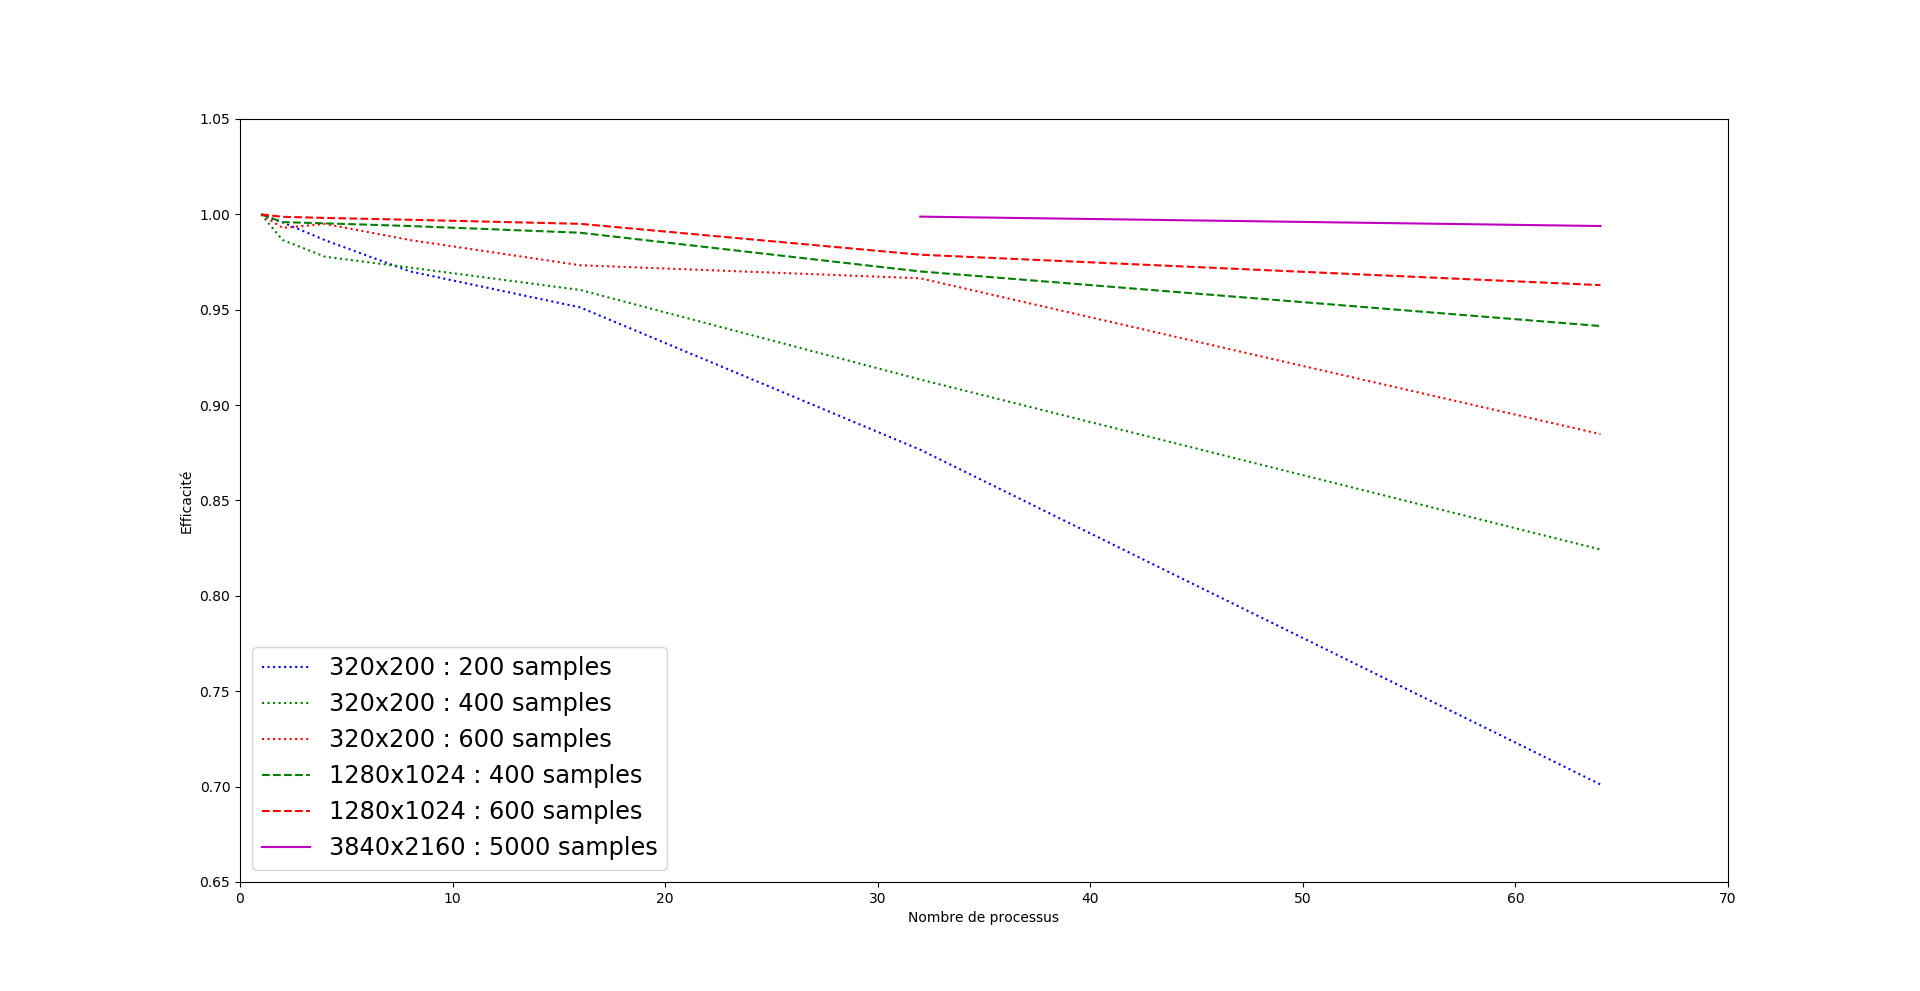
\includegraphics[scale=0.4, center]{temps_partie1.png}
  \caption{Courbe de l'efficacit\'e en fonction du nombre de processus pour diff\'erentes tailles d'image}
\end{figure} 


\subsubsection{Analyse}

\paragraph{Petite image : $320 \times 200$}
Comme on peut le voir, on obtient une efficacit\'e de plus de 95\% pour tous les cas avec 20 processus ou moins. 
L'efficacit\'e baisse ensuite d\^u au fait que le nombre de t\^ache initial de chaque processus est tr\`es faible et 
la plupart du temps est pass\'e dans les communications finales.
Ce temps final peut difficilement \^etre r\'eduit. 
On voit bien qu'il n'est pas n\'ecessaire d'utiliser un grand nombre de processus pour une image trop petite.

\paragraph{Image moyenne : $1280 \times 1024$}
Cette fois-ci l'efficacit\'e reste toujours au-dessus de 95\%, l'image est plus longue \`a calculer en s\'equentiel ( plus d'une heure ). On a donc un speed-up quasi-lin\'eaire,
plus de temps est pass\'e dans la partie calcul que dans la partie finale qui n'est pas parall\'elisable.

\paragraph{Grande image : $3840 \times 2160$}
Dans ce cas l\`a, l'image \'etant tellement grande, l'efficacit\'e diminue plus lentement, on a un speed-up lin\'eaire sur les deux tests que nous avons pu faire dans un temps raisonnable.

\subsection{Am\'eliorations possibles}

\paragraph{}
Dans le cadre du projet nous avons fait certains choix et impl\'ementation et nous proposons ici plusieurs possibilit\'ees d'am\'elioration possibles \`a notre programme.

\paragraph{Taille des t\^aches}
On pourrait changer le ratio auquel multiplier le nombre de sample ou utiliser une fonction qui prend en compte d'autres param\`etres (taille de l'image, nombre de processus).

\paragraph{Impl\'ementation du vol}
Dans notre impl\'ementation actuelle, chaque processus ne communique qu'avec une seule victime ou un seul voleur. 
Augmenter cela pour le nombre de voleur am\'eliorerait les performances et probablement de m\^eme pour le nombre de victime mais
compliquerait beaucoup l'impl\'ementation.

\paragraph{Pr\'eparer la r\'ecup\'eration plus t\^ot}
Nous avons pens\'e \`a aussi modifier la condition de vol des lignes en introduisant un concept de p\'enalit\'e.
Cette p\'enalit\'e aurait pour effet de modifier le moment au cours duquel le processus demande des lignes ainsi que la quantit\'e de ligne vol\'ee.
La p\'enalit\'e serait calcul\'ee en fonction du niveau dans l'arbre. 

De cette mani\`ere, les processus haut dans l'arbre auraient un peu plus de lignes \`a calculer, ce qui permettrait aux processus 
bas dans l'arbre de finir plus vite et d'envoyer leurs donn\'ees \`a leurs parents pendant que leur parent fini ses calculs.

\newpage

\section{Parall\'elisation OpenMPI + OpenMP}

\subsection{Sections parall\`eles}
\paragraph{}
Pour cette partie, nous avons d'abord cherch\'e dans notre algortihme quelles \'etaient les parties parall\'elisables et 
corriger l'al\'eatoire n'\'etant pas thread-safe. 

Dans l'algorithme du path-tracer, pour calculer la valeur finale d'un pixel, les valeurs de 4 sous-pixels sont calcul\'ees et moyenn\'ees. 
Les valeurs de ces 4 sous-pixels sont les moyennes des rayons qui sont consid\'er\'es comme des samples.

Afin d'am\'eliorer les performances du multithread, nous avons modifié certaines parties du calcul des pixels sans que cela ne change la validité du résultat.
Par exemple, \`a la fin du calcul d'un sample, on ajoute dans le r\'esultat du sous-pixel la valeur calcul\'ee pour ce sample avec la formule $\frac{1}{\text{nombre de samples}} \times \text{valeur}$ (afin de donner à chaque valeur calculée une importance de 1 / samples). Au lieu de faire cela, on ajoute dans des variables temporaires les valeurs calcul\'ees dans un tour de boucle, puis apr\`es la boucle, on divise par samples.
Cela permet donc d'\'eviter de faire samples divisions, celle-ci étant beaucoup plus co\^uteuse qu'une addition.

\subsection{Section parall\'elisable}
\paragraph{Sample}
Nous avons premi\`erement testé de parall\'elis\'er la boucle qui g\'en\`ere les rayons samples. 

\paragraph{Sous-pixels}
Nous avons ensuite testé de parall\'elis\'er en donnant un sous-pixel par thread. 

\paragraph{Pixels}
Nous avons enfin testé de parall\'elis\'er la boucle en donnant un pixel entier \`a calculer par thread. 

\subsection{Changement d'al\'ea}
\paragraph{}
\`A chaque besoin de nombre al\'eatoire, le programme utilise actuellement la fonction erand48().
Cependant, la fonction n'est pas thread-safe car elle modifie des variables globales et les lis en m\^eme temps. Il est donc n\'ecessaire de changer la fonction utilis\'e.
Pour cela, nous utilisons la fonction rand\_r() qui g\'en\`ere un entier non sign\'e al\'eatoire entre 0 et une valeur RAND\_MAX. Pour obtenir ensuite un nombre entre
0 et 1, on divise le r\'esultat par RAND\_MAX.

D'autres options ont \'et\'e envisag\'ees, comme utiliser la librairie random, mais celle-ci semblait la plus rapide. 
Etant donn\'ee que l'al\'eatoire n'est pas utilis\'e de mani\`ere cryptographique, il n'est pas nécessaire que l'on utilise une fonction pseudo-aléatoire efficace. Nous sommes donc r\'est\'e sur cette m\'ethode.

\subsection{Mesures et performances}
\paragraph{}
Pour mesurer les qualit\'es des parall\'elisations impl\'ement\'ees, nous allons comparer le temps pass\'e dans la fonction 
comportant le multithread avec la fonction avec un seul thread.

Les communications ne faisant pas partie de notre partie parall\'elisable, 
on ex\'ecutera le programme que sur deux machines en variant le nombre de noeud et les dimensions et nombre de samples de l'image.

La parall\'elisation OpenMP a d'abord \'et\'e test\'e sur le code s\'equentiel. 
M\^eme sur le code s\'equentiel, nous n'avons pas obtenu une acc\'el\'eration de 2 ou sup\'erieur avec 2 threads. 
Nous avons alors cherch\'e la meilleure solutions parmis nos essais.


\begin{figure}[h!]
  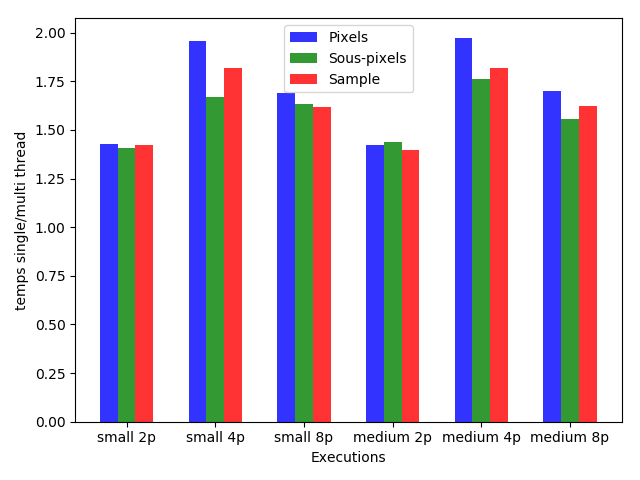
\includegraphics[scale=0.5, center]{rapports_partie2-1.png}
  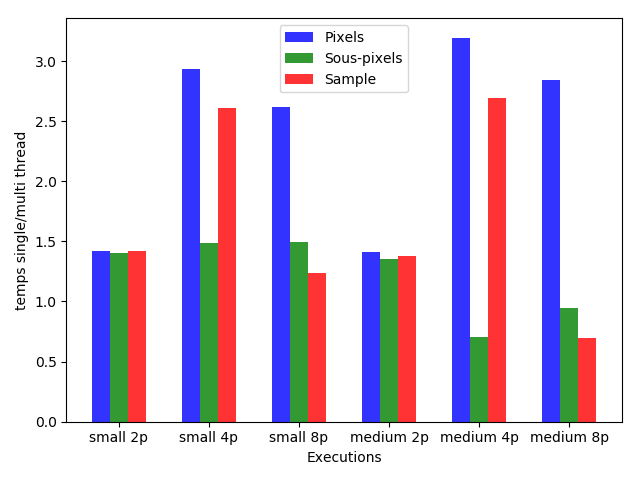
\includegraphics[scale=0.5, center]{rapports_partie2-2.png}
  \caption{Rapport des temps entre une execution sans thread et une execution avec 2 threads puis avec une execution avec 4 threads pour deux images et different nombres de processus}
\end{figure} 

\subsection{Analyse}

\paragraph{Remarques}
Comme on peut l'observer, le temps multithread peut \^etre tr\`es diff\'erent d'une execution \`a une autre. 
Nous avons eu quelques remarques suite \`a nos mesures : 
\begin{itemize}
    \item Dans aucun des test nous n'avons eu une am\'elioration pour 2 processus en passant de 2 \`a 4 threads, alors qu'on peut en observer une dans les m\^emes conditions pour 4 et 8 processus.
    \item Comme dit pr\'ec\'edemment, nous n'avons pas d'acc\'el\'eration lin\'eaire en passant en multithread. Nous pensons que cela est d\^u \`a la cr\'eation de thread qui peut \^etre lente sur les machines.
    \item Les temps de calcul pour la partie sans thread augmente quand on augmente le nombre de thread alors que cela ne devrait pas l'affecter. Cela est probablement d\^u au syst\`eme qui parall\'elise la destruction de thread.
    \item \'Etant donn\'e que nous avons effectu\'e nos calculs sur la fin du projet, beaucoup d'autres groupes les faisaient aussi en même temps, ce qui peut fausser plusieurs calculs et ex\'ecutions.
\end{itemize}

\paragraph{Multithread sur les samples}
Le probl\`eme de cette m\'ethode est qu'elle d\'epend beaucoup du nombre de sample et avec les param\`etres actuels, un sample est tr\`es rapide \`a calculer. 
Il n'est pas rentable d'en faire une t\^ache, et r\'epartir un thread par it\'eration est moins performant que la parall\'elisation sur les pixels.

\paragraph{Multithread sur les sous-pixels}
On a cette fois-ci un probl\`eme de concurrence lorsqu'on veut le faire en t\^ache, ce qui ralenti l'execution. En utilisant un for, l'am\'elioration est moins importante que sur les pixels.
Une optimisation est s\^urement possible mais il faudrait alors changer certaines variables et demanderait beaucoup de test.

\paragraph{Multithread sur les pixels}
Comme notre algorithme cr\'e\'e des t\^aches avec un nombre variable de pixel, pour les test que nous avons fait, c'est la meilleur m\'ethode. 
Dans le cas d'une grande image avec plusieurs threads, on pourra augmenter la taille des t\^aches.

\newpage

\section{Parall\'elisation SIMD}

\subsection{Via OpenMP}
\paragraph{}
Nous avons d'abord cherch\'e quelles \'etaient les parties que l'on pouvait vectoriser sans modifier sensiblement le code initial, \`a part mettre des tableaux en align\'e et d\'eclarer des fonctions en SIMD. Malheureusement, le code de calcul de base n'est pas vraiment "vectorisable". Nous avons quand m\^eme tent\'e d'utiliser des pragma omp simd (for), et les r\'esultats ne sont pas significatifs, on ne gagne que quelques secondes. Sur les trois parties de parallélisation identifi\'ees auparavent, le SIMD via OpenMP ne change que tr\`es peu les r\'esultats.

\subsection{Via les fonctions intrins\`eques}
\paragraph{}
Nous avons ensuite \'etudi\'e l'utilisation des fonctions intrins\`eques. 
On peut voir qu'il n'est pas du tout optimal d'utiliser les fonctions intrins\`eques sur plusieurs samples en m\^eme temps, un sample rentre un nombre al\'eatoire de fois dans la fonction radiance. 
La seule option est donc d'optimiser les calcul en mettant les coordonn\'ees dans un avx soit 3 doubles. On pourrait alors acc\'el\'erer alors 3 fois. Cependant, les calculs n'\'etant pas toujours simples,
on doit utiliser beaucoup de "techniques" pour les faire en avx ( permutation d'avx ).

\paragraph{}
Dans plusieurs des fonctions que l'on doit modifier en avx, on se rend compte qu'il faut faire des op\'erations en plus, notamment pour le produit en croix ou autres.
Cela entra\^ine aussi une modification cons\'equente du code. Nous avons modifi\'e tout en avx dans la boucle sample sauf la fonction radiance qui castera les avx en double et inversement.
Cela cr\'eer beaucoup de chargement que l'on pourrait modifier pour am\'eliorer. Il y a aussi le fait que le code repose beaucoup sur des modifications de variable gr\^ace aux pointeurs, ce qui
ne correspond pas \`a une utilisation des fonctions intrins\`eques.


\newpage

\appendix
\section{Test de performance OpenMPI}

\label{temps partie1}

\paragraph{}
Pour les calculs des accélérations (Speedup) et efficacité (Efficiency), 
nous avons utilisé les formules suivantes : \\
Soit $p$ le nombre de processus,
$T_k(n)$ le temps de d'exécution de l'algorithme sur un problème de taille $n$ avec $k$ processus,
$S(n,p)$ l'accélération et $E(n,p)$ l'efficacité.
$$
  S(n,p) = \frac{T_1(n)}{T_p(n)}
  ,
  E(n,p) = \frac{S(n,p)}{p}
$$

\paragraph{}
Tous nos tests ont été effectués sur les machines de la salle 14-406 de la ppti.
Les temps actuels ont \'et\'e mesur\'es en additionnant les temps de calcul.

\subsection{Petite image}

\subsubsection{200 samples}

\begin{tabular}{ | c | c | c | c |}
  \hline
  Processus & Temps (en s) & Accélération & Efficacité \\
  \hline
  1 & 177.90 & $\frac{177.87}{177.90} = 1.00 $ & $ \frac{1.00}{1} = 100\% $ \\
  2 & 88.89 & $\frac{177.03}{88.89} = 1.99 $ & $ \frac{1.99}{2} = 100\% $ \\
  4 & 44.92 & $\frac{177.26}{44.92} = 3.95 $ & $ \frac{3.95}{4} = 99\% $ \\
  8 & 22.82 & $\frac{177.07}{22.82} = 7.76 $ & $ \frac{7.76}{8} = 97\% $ \\
  16 & 11.66 & $\frac{177.40}{11.66} = 15.21 $ & $ \frac{15.21}{16} = 95\% $ \\
  32 & 6.46 & $\frac{181.16}{6.46} = 28.04 $ & $ \frac{28.04}{32} = 88\% $ \\
  64 & 4.14 & $\frac{185.70}{4.14} = 44.86 $ & $ \frac{44.86}{64} = 70\% $ \\
  \hline
\end{tabular}

\subsubsection{400 samples}

\begin{tabular}{ | c | c | c | c |}
  \hline
  Processus & Temps (en s) & Accélération & Efficacité \\
  \hline
  1 & 360.20 & $\frac{360.17}{360.20} = 1.00 $ & $ \frac{1.00}{1} = 100\% $ \\
  2 & 179.94 & $\frac{355.05}{179.94} = 1.97 $ & $ \frac{1.97}{2} = 98\% $ \\
  4 & 90.64 & $\frac{354.49}{90.64} = 3.91 $ & $ \frac{3.91}{4} = 98\% $ \\
  8 & 45.55 & $\frac{354.20}{45.55} = 7.78 $ & $ \frac{7.78}{8} = 97\% $ \\
  16 & 23.07 & $\frac{354.41}{23.07} = 15.36 $ & $ \frac{15.36}{16} = 96\% $ \\
  32 & 12.34 & $\frac{360.75}{12.34} = 29.23 $ & $ \frac{29.23}{32} = 91\% $ \\
  64 & 7.00 & $\frac{369.39}{7.00} = 52.77 $ & $ \frac{52.77}{64} = 82\% $ \\
  \hline
\end{tabular}

\subsubsection{600 samples}

\begin{tabular}{ | c | c | c | c |}
  \hline
  Processus & Temps (en s) & Accélération & Efficacité \\
  \hline
  1 & 537.23 & $\frac{537.20}{537.23} = 1.00 $ & $ \frac{1.00}{1} = 100\% $ \\
  2 & 269.75 & $\frac{535.65}{269.75} = 1.99 $ & $ \frac{1.99}{2} = 100\% $ \\
  4 & 133.61 & $\frac{531.78}{133.61} = 3.98 $ & $ \frac{3.98}{4} = 100\% $ \\
  8 & 67.36 & $\frac{531.62}{67.36} = 7.89 $ & $ \frac{7.89}{8} = 99\% $ \\
  16 & 34.15 & $\frac{531.78}{34.15} = 15.57 $ & $ \frac{15.57}{16} = 97\% $ \\
  32 & 17.50 & $\frac{541.33}{17.50} = 30.93 $ & $ \frac{30.93}{32} = 97\% $ \\
  64 & 9.78 & $\frac{553.80}{9.78} = 56.63 $ & $ \frac{56.63}{64} = 88\% $ \\
  \hline
\end{tabular}

\subsection{Moyenne image}

\subsubsection{400 samples}

\begin{tabular}{ | c | c | c | c |}
  \hline
  Processus & Temps (en s) & Accélération & Efficacité \\
  \hline
  1 & 10282.23 & $\frac{10281.55}{10282.23} = 1.00 $ & $ \frac{1.00}{1} = 100\% $ \\
  2 & 4496.40 & $\frac{8955.99}{4496.40} = 1.99 $ & $ \frac{1.99}{2} = 100\% $ \\
  4 & 2002.48 & $\frac{7971.99}{2002.48} = 3.98 $ & $ \frac{3.98}{4} = 100\% $ \\
  8 & 1002.56 & $\frac{7971.26}{1002.56} = 7.95 $ & $ \frac{7.95}{8} = 99\% $ \\
  16 & 502.05 & $\frac{7955.12}{502.05} = 15.85 $ & $ \frac{15.85}{16} = 99\% $ \\
  32 & 259.70 & $\frac{8061.56}{259.70} = 31.04 $ & $ \frac{31.04}{32} = 97\% $ \\
  64 & 138.22 & $\frac{8328.34}{138.22} = 60.25 $ & $ \frac{60.25}{64} = 94\% $ \\
  \hline
\end{tabular}

\subsubsection{600 samples}

\begin{tabular}{ | c | c | c | c |}
  \hline
  Processus & Temps (en s) & Accélération & Efficacité \\
  \hline
  8 & 1516.89 & $\frac{12100.28}{1516.89} = 7.98 $ & $ \frac{7.98}{8} = 100\% $ \\
  16 & 759.57 & $\frac{12092.56}{759.57} = 15.92 $ & $ \frac{15.92}{16} = 100\% $ \\
  32 & 390.87 & $\frac{12242.99}{390.87} = 31.32 $ & $ \frac{31.32}{32} = 98\% $ \\
  64 & 222.28 & $\frac{13697.52}{222.28} = 61.62 $ & $ \frac{61.62}{64} = 96\% $ \\
  \hline
\end{tabular}

\subsection{Grande image}

\begin{tabular}{ | c | c | c | c |}
  \hline
  Processus & Temps (en s) & Accélération & Efficacité \\
  \hline
  32 & 17352.68 & $\frac{554608.03}{17352.68} = 31.96 $ & $ \frac{31.96}{32} = 100\% $ \\
  64 & 8936.92 & $\frac{568448.44}{8936.92} = 63.61 $ & $ \frac{63.61}{64} = 99\% $ \\
  \hline
\end{tabular}

\section{Test de performance OpenMPI + OpenMP}

\paragraph{}
Les calculs des rapports sont pond\'er\'es par le nombre de t\^ache termin\'ee que nous n'affichons
pas dans ces tableaux mais qui sont disponible dans le dossier temps.

\subsection{Sample}

\subsubsection{Small image}

\begin{tabular}{ | c | c | c | c | c | }
  \hline
  Processus & Thread & Temps single thread & Temps multi thread & Rapport \\
  \hline
  2 & 2 & 846.66 & 596.56 & $ \frac{846.66}{596.56} = 1.42 $ \\
  2 & 4 & 846.63 & 596.72 & $ \frac{846.63}{596.72} = 1.42 $ \\
  4 & 2 & 861.15 & 474.06 & $ \frac{861.15}{474.06} = 1.82 $ \\
  4 & 4 & 881.40 & 337.46 & $ \frac{881.40}{337.46} = 2.61 $ \\
  8 & 2 & 970.17 & 600.77 & $ \frac{970.17}{600.77} = 1.61 $ \\
  8 & 4 & 1093.48 & 889.78 & $ \frac{1093.48}{889.78} = 1.23 $ \\
  \hline
\end{tabular}


\subsubsection{Medium image}

\begin{tabular}{ | c | c | c | c | c | }
  \hline
  Processus & Thread & Temps single thread & Temps multi thread & Rapport \\
  \hline
  2 & 2 & 1880.24 & 1348.96 & $ \frac{1880.24}{1348.96} = 1.39 $ \\
  2 & 4 & 1885.66 & 1367.35 & $ \frac{1885.66}{1367.35} = 1.38 $ \\
  4 & 2 & 1927.77 & 1060.36 & $ \frac{1927.77}{1060.36} = 1.82 $ \\
  4 & 4 & 1986.12 & 738.04 & $ \frac{1986.12}{738.04} = 2.69 $ \\
  8 & 2 & 2180.95 & 1344.71 & $ \frac{2180.95}{1344.71} = 1.62 $ \\
  8 & 4 & 2485.71 & 3580.70 & $ \frac{2485.71}{3580.70} = 0.69 $ \\
  \hline
\end{tabular}


\subsection{Sous-pixels}

\subsubsection{Small image}

\begin{tabular}{ | c | c | c | c | c | }
  \hline
  Processus & Thread & Temps single thread & Temps multi thread & Rapport \\
  \hline
  2 & 2 & 896.46 & 637.15 & $ \frac{896.46}{637.15} = 1.41 $ \\
  2 & 4 & 851.30 & 606.50 & $ \frac{851.30}{606.50} = 1.40 $ \\
  4 & 2 & 1007.31 & 605.14 & $ \frac{1007.31}{605.14} = 1.66 $ \\
  4 & 4 & 1266.19 & 854.71 & $ \frac{1266.19}{854.71} = 1.48 $ \\
  8 & 2 & 1052.16 & 645.38 & $ \frac{1052.16}{645.38} = 1.63 $ \\
  8 & 4 & 1255.64 & 845.01 & $ \frac{1255.64}{845.01} = 1.49 $ \\
  \hline
\end{tabular}

\subsubsection{Medium image}

\begin{tabular}{ | c | c | c | c | c | }
  \hline
  Processus & Thread & Temps single thread & Temps multi thread & Rapport \\
  \hline
  2 & 2 & 2078.70 & 1447.78 & $ \frac{2078.70}{1447.78} = 1.44 $ \\
  2 & 4 & 1986.92 & 1469.30 & $ \frac{1986.92}{1469.30} = 1.35 $ \\
  4 & 2 & 2002.06 & 1137.44 & $ \frac{2002.06}{1137.44} = 1.76 $ \\
  4 & 4 & 3673.02 & 5242.87 & $ \frac{3673.02}{5242.87} = 0.70 $ \\
  8 & 2 & 2162.99 & 1392.78 & $ \frac{2162.99}{1392.78} = 1.55 $ \\
  8 & 4 & 2491.76 & 2633.93 & $ \frac{2491.76}{2633.93} = 0.95 $ \\
  \hline
\end{tabular}


\subsection{Pixels}

\subsubsection{Small image}

\begin{tabular}{ | c | c | c | c | c | }
  \hline
  Processus & Thread & Temps single thread & Temps multi thread & Rapport \\
  \hline
  2 & 2 & 845.79 & 593.40 & $ \frac{845.79}{593.40} = 1.43 $ \\
  2 & 4 & 844.33 & 594.07 & $ \frac{844.33}{594.07} = 1.42 $ \\
  4 & 2 & 857.59 & 439.71 & $ \frac{857.59}{439.71} = 1.95 $ \\
  4 & 4 & 877.48 & 298.80 & $ \frac{877.48}{298.80} = 2.94 $ \\
  8 & 2 & 967.96 & 574.03 & $ \frac{967.96}{574.03} = 1.69 $ \\
  8 & 4 & 1056.97 & 405.75 & $ \frac{1056.97}{405.75} = 2.60 $ \\
  \hline
\end{tabular}

\subsubsection{Medium image}

\begin{tabular}{ | c | c | c | c | c | }
  \hline
  Processus & Thread & Temps single thread & Temps multi thread & Rapport \\
  \hline
  2 & 2 & 1887.11 & 1326.92 & $ \frac{1887.11}{1326.92} = 1.42 $ \\
  2 & 4 & 1878.08 & 1332.27 & $ \frac{1878.08}{1332.27} = 1.41 $ \\
  4 & 2 & 1923.49 & 975.08 & $ \frac{1923.49}{975.08} = 1.97 $ \\
  4 & 4 & 1973.38 & 619.04 & $ \frac{1973.38}{619.04} = 3.19 $ \\
  8 & 2 & 2157.21 & 1271.22 & $ \frac{2157.21}{1271.22} = 1.70 $ \\
  8 & 4 & 2388.96 & 840.17 & $ \frac{2388.96}{840.17} = 2.84 $ \\
  \hline
\end{tabular}

\end{document}
